%%%%%%%%%%%%%%%%%%%%%%%%%%%%%%%%%%%%%%%%%%%%%%%%%%%%%%%%%%%%%%%%%%%%%%%%
% Plantilla TFG/TFM
% Escuela Politécnica Superior de la Universidad de Alicante
% Realizado por: Jose Manuel Requena Plens
% Contacto: info@jmrplens.com / Telegram:@jmrplens
%%%%%%%%%%%%%%%%%%%%%%%%%%%%%%%%%%%%%%%%%%%%%%%%%%%%%%%%%%%%%%%%%%%%%%%%

\chapter{Marco Teórico}
\label{marcoteorico}

\section{Predicción económica y series temporales}

La predicción económica constituye una herramienta fundamental para el análisis y la toma de decisiones en ámbitos como la política económica, la planificación empresarial o la evaluación del ciclo económico. En este contexto, muchas de las variables de interés, como el Producto Interior Bruto (PIB), la inflación o el empleo, se observan de forma periódica y ordenada en el tiempo, dando lugar a lo que se conoce como series temporales económicas.

Una serie temporal se define como una secuencia de observaciones de una variable registradas a lo largo del tiempo, donde el orden temporal y la dependencia entre observaciones consecutivas desempeñan un papel clave. A diferencia de otros tipos de datos, en las series temporales el valor observado en un momento determinado suele depender de valores anteriores de la misma variable, lo que introduce una estructura de dependencia temporal que debe ser considerada en los procesos de análisis y predicción.

Las series temporales económicas suelen presentar características específicas como tendencias, estacionalidad y persistencia. La tendencia hace referencia a la evolución de largo plazo de una variable, reflejando cambios estructurales en la economía. La estacionalidad, por su parte, recoge patrones que se repiten de forma periódica dentro de un mismo año, como puede ocurrir con ciertos indicadores de consumo o producción. Finalmente, la persistencia o dependencia temporal refleja la influencia que los valores pasados de una variable pueden tener sobre sus valores futuros. Estas características condicionan los enfoques utilizados para el análisis y la predicción de las series económicas. \citep{hyndman_athanasopoulos_fpp3}

En el ámbito de la predicción macroeconómica, el objetivo principal consiste en estimar el valor futuro de una variable a partir de la información disponible en el pasado. Para ello, es habitual utilizar tanto la propia historia de la variable que se desea predecir como otras variables económicas relacionadas que puedan aportar información relevante sobre su evolución futura.

Sin embargo, la predicción económica presenta importantes dificultades. Las economías están sujetas a cambios estructurales, shocks externos y comportamientos complejos de los agentes económicos, lo que puede alterar las relaciones entre variables a lo largo del tiempo. Además, la disponibilidad de datos suele ser limitada en comparación con otros ámbitos de aplicación del análisis de datos, especialmente cuando se trabaja con variables agregadas de carácter macroeconómico.

En este escenario, la predicción económica se plantea como un problema complejo que requiere un equilibrio entre simplicidad, capacidad explicativa y precisión predictiva. Este hecho ha motivado el desarrollo y la comparación de distintos enfoques de predicción, desde modelos sencillos de referencia hasta técnicas más avanzadas, con el objetivo de mejorar la capacidad para anticipar la evolución futura de las principales variables macroeconómicas. \citep{green_armstrong_2015}

Tradicionalmente, la predicción de series temporales económicas se ha abordado mediante modelos estadísticos y econométricos que buscan capturar la estructura temporal de los datos. No obstante, en los últimos años han surgido nuevas aproximaciones basadas en técnicas de aprendizaje automático, que permiten modelizar relaciones más complejas entre variables y aprovechar mejor la información disponible en los datos.

Estas nuevas aproximaciones no sustituyen necesariamente a los métodos tradicionales, sino que en muchos casos actúan como herramientas complementarias. Mientras que los modelos econométricos clásicos suelen centrarse en la interpretación estructural de las relaciones económicas, los modelos de aprendizaje automático priorizan la capacidad predictiva y la detección de patrones en los datos, lo que puede resultar especialmente útil en problemas de predicción económica.

\section{Modelos de aprendizaje automático para predicción económica}

En los últimos años, el desarrollo de técnicas de aprendizaje automático ha abierto nuevas posibilidades para el análisis y la predicción de variables económicas. A diferencia de muchos modelos econométricos tradicionales, que requieren especificar previamente una relación funcional concreta entre variables, los modelos de aprendizaje automático permiten aprender estas relaciones directamente a partir de los datos.

Estas técnicas han demostrado un gran potencial en problemas donde las relaciones entre variables pueden ser complejas, no lineales o difíciles de especificar mediante modelos estadísticos tradicionales. En particular, los algoritmos de aprendizaje supervisado permiten construir modelos predictivos a partir de conjuntos de datos históricos, identificando patrones que pueden utilizarse posteriormente para estimar valores futuros.

En el ámbito de la predicción económica, estas técnicas resultan especialmente interesantes cuando se dispone de múltiples variables explicativas que pueden influir en la evolución de un indicador macroeconómico. Variables como el empleo, la inflación o indicadores de actividad económica pueden aportar información relevante para anticipar la evolución del PIB, aunque la relación exacta entre ellas no siempre sea sencilla de modelizar mediante enfoques tradicionales.

Entre los algoritmos de aprendizaje automático más utilizados en problemas de predicción con datos tabulares se encuentran métodos basados en árboles de decisión y técnicas de ensamblado de modelos (\textit{ensemble learning}). Estos enfoques combinan múltiples modelos simples con el objetivo de mejorar la precisión predictiva y reducir el riesgo de sobreajuste.

Dentro de esta familia de métodos, los algoritmos basados en \textit{boosting} han demostrado un rendimiento especialmente destacado en problemas de predicción con datos estructurados, lo que ha motivado su creciente utilización en distintos ámbitos del análisis de datos.

\section{Gradient Boosting}

El \textit{Gradient Boosting} es una técnica de aprendizaje automático basada en la combinación secuencial de múltiples modelos simples con el objetivo de construir un modelo predictivo más preciso. Este enfoque pertenece a la familia de métodos de ensamblado, cuyo principio fundamental consiste en combinar varios modelos individuales para obtener un rendimiento superior al que se obtendría utilizando un único modelo. \citep{friedman_gradient_boosting_2001, zhou_ensemble_2012}

En el caso del \textit{boosting}, los modelos se construyen de forma secuencial, de modo que cada nuevo modelo intenta corregir los errores cometidos por los modelos anteriores. Habitualmente, estos modelos base son árboles de decisión de baja profundidad, lo que permite capturar relaciones no lineales entre variables sin introducir una complejidad excesiva. \citep{friedman_gradient_boosting_2001}

\begin{figure}[H]
\centering
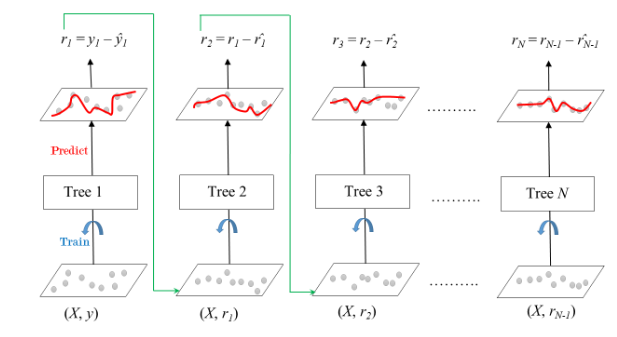
\includegraphics[width=0.9\textwidth]{figures/gradientboosting.png}
\caption{Proceso iterativo de entrenamiento en Gradient Boosting. Cada nuevo árbol se entrena para aproximar los errores residuales del modelo anterior, construyendo progresivamente una predicción más precisa.}
\label{fig:gradient_boosting}
\end{figure}

Como se observa en la figura \ref{fig:gradient_boosting}, el proceso de entrenamiento comienza con un modelo inicial relativamente simple que realiza una primera aproximación a la variable objetivo. A continuación, se calcula el error cometido por dicho modelo y se entrena un nuevo modelo que intenta explicar ese error. Este proceso se repite de forma iterativa, añadiendo nuevos modelos que van corrigiendo progresivamente los errores residuales de los modelos anteriores. \citep{friedman_gradient_boosting_2001}

El término \textit{gradient} hace referencia al uso del gradiente de la función de pérdida para determinar la dirección en la que debe ajustarse el modelo en cada iteración. En términos generales, el algoritmo busca minimizar una función de pérdida que mide la diferencia entre las predicciones del modelo y los valores reales observados. \citep{friedman_gradient_boosting_2001}

Este enfoque permite construir modelos muy flexibles capaces de capturar relaciones complejas entre variables, lo que explica su buen rendimiento en numerosos problemas de predicción. No obstante, también requiere un control cuidadoso de parámetros como la profundidad de los árboles o la tasa de aprendizaje para evitar problemas de sobreajuste.

\section{XGBoost}

XGBoost (\textit{Extreme Gradient Boosting}) es una implementación optimizada del algoritmo de \textit{Gradient Boosting} diseñada para mejorar la eficiencia computacional y el rendimiento predictivo. Este algoritmo ha ganado una gran popularidad en el ámbito del aprendizaje automático debido a su alto rendimiento en problemas de predicción con datos estructurados.

Una de las principales características de XGBoost es la incorporación de técnicas de regularización que permiten controlar la complejidad del modelo y reducir el riesgo de sobreajuste. A diferencia de implementaciones más básicas de \textit{boosting}, XGBoost incluye términos de penalización que limitan el crecimiento excesivo de los árboles de decisión y favorecen modelos más robustos. \citep{chen_guestrin_2016}

Además, XGBoost introduce diversas mejoras en términos de eficiencia computacional, como el uso de paralelización en el entrenamiento, optimizaciones en el manejo de memoria y técnicas avanzadas para el procesamiento de datos. Estas características permiten entrenar modelos de forma rápida incluso cuando se trabaja con conjuntos de datos relativamente grandes. \citep{chen_guestrin_2016}

En el contexto de la predicción económica, XGBoost resulta especialmente adecuado para trabajar con datos tabulares que incluyen múltiples variables explicativas. Su capacidad para capturar relaciones no lineales y efectos de interacción entre variables lo convierte en una herramienta potente para analizar la relación entre distintos indicadores macroeconómicos y la evolución del PIB. \citep{chen_guestrin_2016}

Por estas razones, XGBoost ha sido ampliamente utilizado en distintos ámbitos del análisis de datos y ha demostrado un alto rendimiento en competiciones de aprendizaje automático y aplicaciones reales. Su equilibrio entre capacidad predictiva, eficiencia computacional y control del sobreajuste lo convierte en una opción especialmente atractiva para problemas de predicción económica. La Figura~\ref{fig:decision_tree} muestra la estructura interna de un árbol de decisión individual de profundidad 3, el tipo de modelo base que emplea XGBoost.

\begin{figure}[H]
\centering
\resizebox{\linewidth}{!}{%
\begin{tikzpicture}[
  nodo/.style={draw, rounded corners=3pt, fill=blue!10, minimum width=1.8cm,
               minimum height=0.75cm, align=center, font=\small},
  hoja/.style={draw, rounded corners=3pt, fill=green!15, minimum width=1.2cm,
               minimum height=0.65cm, align=center, font=\small},
  arr/.style={->, >=stealth, thick},
  etiq/.style={font=\scriptsize, inner sep=2pt}
]

% --- Nivel 0 (raíz) ---
\node[nodo] (n0) {$x_1 < \theta_1$};

% --- Nivel 1 ---
\node[nodo, below left=1.0cm and 1.6cm of n0]  (n1l) {$x_2 < \theta_2$};
\node[nodo, below right=1.0cm and 1.6cm of n0] (n1r) {$x_3 < \theta_3$};

% --- Nivel 2 ---
\node[nodo, below left=0.9cm and 0.4cm of n1l]  (n2ll) {$x_4 < \theta_4$};
\node[nodo, below right=0.9cm and 0.4cm of n1l] (n2lr) {$x_5 < \theta_5$};
\node[nodo, below left=0.9cm and 0.4cm of n1r]  (n2rl) {$x_6 < \theta_6$};
\node[nodo, below right=0.9cm and 0.4cm of n1r] (n2rr) {$x_7 < \theta_7$};

% --- Nivel 3 (hojas) ---
\node[hoja, below left=0.8cm and 0.1cm of n2ll]  (h1) {$\hat{y}_1$};
\node[hoja, below right=0.8cm and 0.1cm of n2ll] (h2) {$\hat{y}_2$};
\node[hoja, below left=0.8cm and 0.1cm of n2lr]  (h3) {$\hat{y}_3$};
\node[hoja, below right=0.8cm and 0.1cm of n2lr] (h4) {$\hat{y}_4$};
\node[hoja, below left=0.8cm and 0.1cm of n2rl]  (h5) {$\hat{y}_5$};
\node[hoja, below right=0.8cm and 0.1cm of n2rl] (h6) {$\hat{y}_6$};
\node[hoja, below left=0.8cm and 0.1cm of n2rr]  (h7) {$\hat{y}_7$};
\node[hoja, below right=0.8cm and 0.1cm of n2rr] (h8) {$\hat{y}_8$};

% --- Flechas nivel 0 → 1 ---
\draw[arr] (n0.south) -- (n1l.north) node[etiq, midway, above left]{sí};
\draw[arr] (n0.south) -- (n1r.north) node[etiq, midway, above right]{no};

% --- Flechas nivel 1 → 2 ---
\draw[arr] (n1l.south) -- (n2ll.north) node[etiq, midway, above left]{sí};
\draw[arr] (n1l.south) -- (n2lr.north) node[etiq, midway, above right]{no};
\draw[arr] (n1r.south) -- (n2rl.north) node[etiq, midway, above left]{sí};
\draw[arr] (n1r.south) -- (n2rr.north) node[etiq, midway, above right]{no};

% --- Flechas nivel 2 → hojas ---
\draw[arr] (n2ll.south) -- (h1.north);
\draw[arr] (n2ll.south) -- (h2.north);
\draw[arr] (n2lr.south) -- (h3.north);
\draw[arr] (n2lr.south) -- (h4.north);
\draw[arr] (n2rl.south) -- (h5.north);
\draw[arr] (n2rl.south) -- (h6.north);
\draw[arr] (n2rr.south) -- (h7.north);
\draw[arr] (n2rr.south) -- (h8.north);

% --- Anotación de profundidad ---
\node[left=0.3cm of n0,    font=\scriptsize, text=gray] {prof.\ 0};
\node[left=0.3cm of n1l,   font=\scriptsize, text=gray] {prof.\ 1};
\node[left=0.3cm of n2ll,  font=\scriptsize, text=gray] {prof.\ 2};
\node[left=0.3cm of h1,    font=\scriptsize, text=gray] {prof.\ 3};

\end{tikzpicture}}%
\caption{Estructura de un árbol de decisión de profundidad \texttt{max\_depth=3}. Cada nodo interno evalúa una condición sobre una variable $x_j$ y un umbral $\theta$; las hojas (en verde) contienen la predicción $\hat{y}$ para los ejemplos que alcanzan ese nodo.}
\label{fig:decision_tree}
\end{figure}